% Equation flow of the base paper (Golestani et al., IEEE Access 2022), blocks 1-6.
% Build:  pdflatex flow_paper.tex
\documentclass[border=10pt]{standalone}
\usepackage{tikz}
% Shared preamble of the two flow diagrams (flow_paper.tex, flow_x3.tex)
\usepackage{amsmath,amssymb,bm}
\usepackage[most]{tcolorbox}
\usetikzlibrary{positioning,arrows.meta,calc,fit,backgrounds}
\definecolor{cPlant}{HTML}{37474F}
\definecolor{cEnv}{HTML}{A0620F}
\definecolor{cCtrl}{HTML}{AD1457}
\definecolor{cAdapt}{HTML}{4527A0}
\definecolor{cX3}{HTML}{1565C0}
\definecolor{cOk}{HTML}{2E7D32}
\definecolor{cText}{HTML}{263238}
\definecolor{cRef}{HTML}{546E7A}
\newcommand{\vq}{\bm{q}}  \newcommand{\qv}{\bm{q}_v} \newcommand{\vw}{\bm{\omega}}
\newcommand{\vu}{\bm{u}}  \newcommand{\vd}{\bm{d}}   \newcommand{\vs}{\bm{s}}
\newcommand{\vtau}{\bm{\tau}} \newcommand{\veps}{\bm{\varepsilon}} \newcommand{\vF}{\bm{F}}
\newcommand{\vp}{\bm{p}}  \newcommand{\vv}{\bm{v}}
\newcommand{\that}{\hat{\theta}}
\newcommand{\sat}{\operatorname{sat}}
\newcommand{\R}{\mathbb{R}}
% \fblock{name}{position}{colour}{number}{title}{equations}{IN}{OUT}
\newcommand{\fblock}[8]{%
  \node[inner sep=0pt, outer sep=0pt] (#1) at #2 {%
  \begin{tcolorbox}[enhanced, width=8.4cm, colback=white, colframe=#3, colbacktitle=#3, coltitle=white,
     title={\sffamily\bfseries\small\tcbox[on line, colback=white, colframe=white, colupper=#3, arc=5pt,
     boxsep=0pt, left=2.5pt, right=2.5pt, top=0.5pt, bottom=0.5pt]{#4}\ #5}, boxrule=0.8pt, arc=3pt,
     left=5pt, right=5pt, top=4pt, bottom=4pt, colbacklower=#3!7, segmentation style={draw=#3!45},
     fontupper=\small, fontlower=\scriptsize\sffamily\color{cText}]
  \centering #6
  \tcblower\raggedright\textbf{IN}\enspace #7\par\smallskip\textbf{OUT}\enspace #8
  \end{tcolorbox}};}
\tikzset{
  sig/.style={-{Stealth[length=2.6mm]}, line width=0.9pt, color=cText},
  lbl/.style={font=\scriptsize\sffamily, text=cText, fill=white, inner sep=1.6pt, align=center},
  aux/.style={draw=cRef, fill=cRef!6, rounded corners=3pt, line width=0.7pt,
              font=\scriptsize\sffamily, text=cText, align=center, inner sep=5pt},
}

\begin{document}
\sffamily
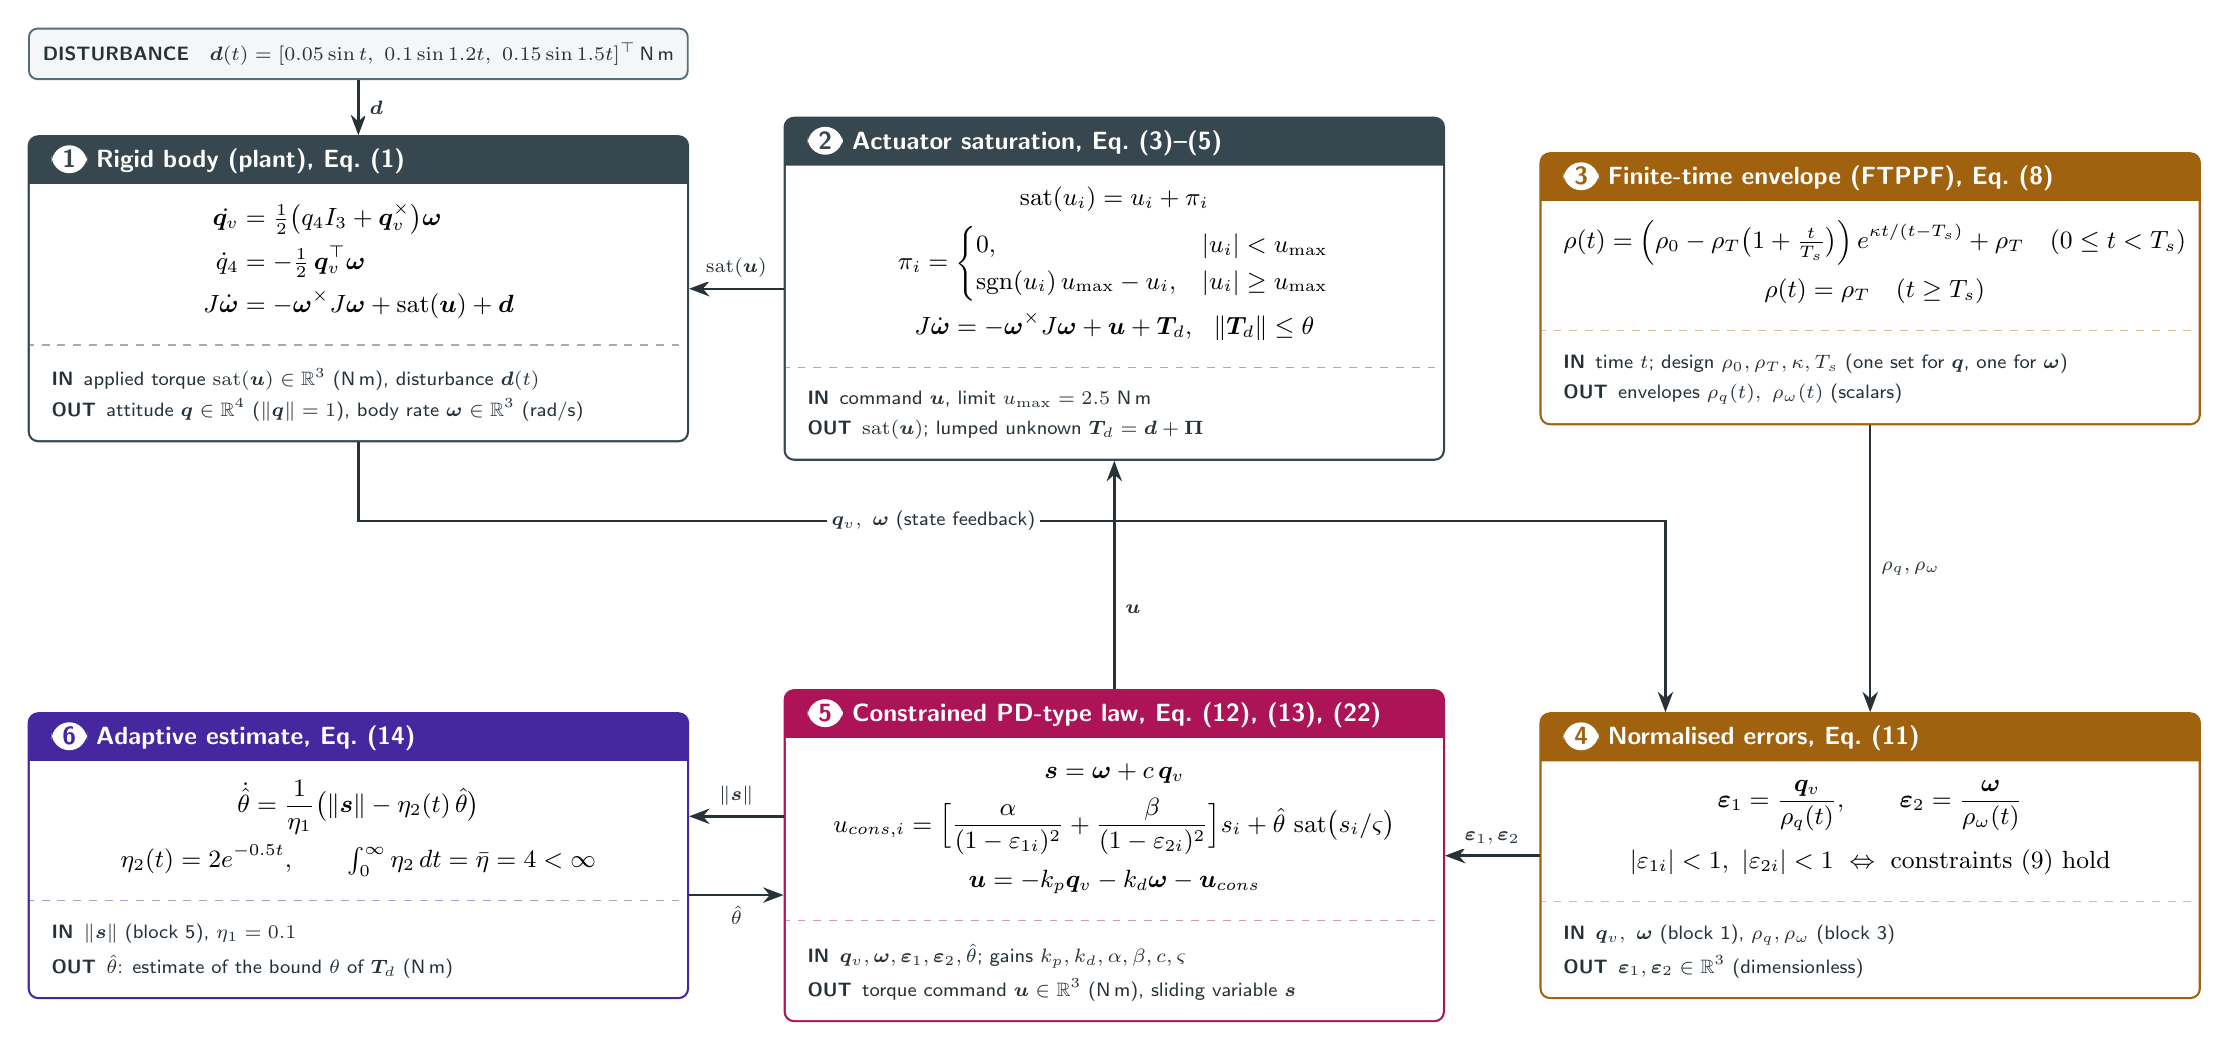
\begin{tikzpicture}
\fblock{b1}{(0,0)}{cPlant}{1}{Rigid body (plant), Eq.~(1)}{%
  $\begin{aligned}\dot{\qv}&=\tfrac12\big(q_4 I_3+\qv^{\times}\big)\vw\\ \dot q_4&=-\tfrac12\,\qv^{\top}\vw\\
   J\dot{\vw}&=-\vw^{\times}J\vw+\sat(\vu)+\vd\end{aligned}$}
  {applied torque $\sat(\vu)\in\R^3$ (N\,m), disturbance $\vd(t)$}
  {attitude $\vq\in\R^4$ ($\|\vq\|=1$), body rate $\vw\in\R^3$ (rad/s)}
\fblock{b2}{(9.6,0)}{cPlant}{2}{Actuator saturation, Eq.~(3)--(5)}{%
  $\begin{gathered}\sat(u_i)=u_i+\pi_i\\
   \pi_i=\begin{cases}0, & |u_i|<u_{\max}\\ \operatorname{sgn}(u_i)\,u_{\max}-u_i, & |u_i|\ge u_{\max}\end{cases}\\
   J\dot{\vw}=-\vw^{\times}J\vw+\vu+\bm T_d,\ \ \|\bm T_d\|\le\theta\end{gathered}$}
  {command $\vu$, limit $u_{\max}=2.5$ N\,m}
  {$\sat(\vu)$; lumped unknown $\bm T_d=\vd+\bm\Pi$}
\fblock{b3}{(19.2,0)}{cEnv}{3}{Finite-time envelope (FTPPF), Eq.~(8)}{%
  $\begin{gathered}\rho(t)=\Big(\rho_0-\rho_T\big(1+\tfrac{t}{T_s}\big)\Big)\,e^{\kappa t/(t-T_s)}+\rho_T\quad(0\le t<T_s)\\
   \rho(t)=\rho_T\quad(t\ge T_s)\end{gathered}$}
  {time $t$; design $\rho_0,\rho_T,\kappa,T_s$ (one set for $\vq$, one for $\vw$)}
  {envelopes $\rho_q(t),\ \rho_\omega(t)$ (scalars)}
\fblock{b4}{(19.2,-7.2)}{cEnv}{4}{Normalised errors, Eq.~(11)}{%
  $\begin{gathered}\veps_1=\dfrac{\qv}{\rho_q(t)},\qquad \veps_2=\dfrac{\vw}{\rho_\omega(t)}\\[2pt]
   |\varepsilon_{1i}|<1,\ |\varepsilon_{2i}|<1\ \Leftrightarrow\ \text{constraints (9) hold}\end{gathered}$}
  {$\qv,\ \vw$ (block 1), $\rho_q,\rho_\omega$ (block 3)}
  {$\veps_1,\veps_2\in\R^3$ (dimensionless)}
\fblock{b5}{(9.6,-7.2)}{cCtrl}{5}{Constrained PD-type law, Eq.~(12), (13), (22)}{%
  $\begin{gathered}\vs=\vw+c\,\qv\\
   u_{cons,i}=\Big[\dfrac{\alpha}{(1-\varepsilon_{1i})^2}+\dfrac{\beta}{(1-\varepsilon_{2i})^2}\Big]s_i+\that\,\sat\!\big(s_i/\varsigma\big)\\
   \vu=-k_p\qv-k_d\vw-\vu_{cons}\end{gathered}$}
  {$\qv,\vw,\veps_1,\veps_2,\that$; gains $k_p,k_d,\alpha,\beta,c,\varsigma$}
  {torque command $\vu\in\R^3$ (N\,m), sliding variable $\vs$}
\fblock{b6}{(0,-7.2)}{cAdapt}{6}{Adaptive estimate, Eq.~(14)}{%
  $\begin{gathered}\dot{\that}=\dfrac{1}{\eta_1}\big(\|\vs\|-\eta_2(t)\,\that\big)\\
   \eta_2(t)=2e^{-0.5t},\qquad \textstyle\int_0^\infty\eta_2\,dt=\bar\eta=4<\infty\end{gathered}$}
  {$\|\vs\|$ (block 5), $\eta_1=0.1$}
  {$\that$: estimate of the bound $\theta$ of $\bm T_d$ (N\,m)}
\node[aux, anchor=south] (dist) at ($(b1.north)+(0,0.7)$)
  {\textbf{DISTURBANCE}\quad $\vd(t)=[0.05\sin t,\ 0.1\sin1.2t,\ 0.15\sin1.5t]^{\top}$\,N\,m};
\draw[sig] (dist.south) -- node[lbl, right=2pt]{$\vd$} (b1.north);
\draw[sig] (b2.west) -- node[lbl, above=2pt]{$\sat(\vu)$} (b1.east);
\draw[sig] (b3.south) -- node[lbl, right=2pt]{$\rho_q,\rho_\omega$} (b4.north);
\draw[sig] (b4.west) -- node[lbl, above=2pt]{$\veps_1,\veps_2$} (b5.east);
\draw[sig] (b5.north) -- node[lbl, right=2pt, pos=0.35]{$\vu$} (b2.south);
\draw[sig] ($(b5.west)+(0,0.5)$) -- node[lbl, above=2pt]{$\|\vs\|$} ($(b6.east)+(0,0.5)$);
\draw[sig] ($(b6.east)+(0,-0.5)$) -- node[lbl, below=2pt]{$\that$} ($(b5.west)+(0,-0.5)$);
\draw[sig] (b1.south) -- ++(0,-1.0) -| node[lbl, pos=0.22]{$\qv,\ \vw$ (state feedback)} ($(b4.north)+(-2.6,0)$);
\end{tikzpicture}
\end{document}
